\documentclass[aps,prb,twocolumn,superscriptaddress,floatfix,longbibliography]{revtex4-2}

\usepackage{minted}
\usepackage{amsmath,amssymb} % math symbols
\usepackage{bm} % bold math font
\usepackage{graphicx} % for figures
\usepackage{comment} % allows block comments
%\usepackage{ulem} % allows strikeout text, e.g. \sout{text}

\usepackage{textcomp} % This package gives the text quote '

\usepackage{enumitem}
\setlist{noitemsep,leftmargin=*,topsep=0pt,parsep=0pt}

\usepackage{xcolor} % \textcolor{red}{text} will be red for notes
\definecolor{lightgray}{gray}{0.6}
\definecolor{medgray}{gray}{0.4}

\usepackage{hyperref}
\hypersetup{
colorlinks=true,
urlcolor= blue,
citecolor=blue,
linkcolor= blue,
% bookmarks=true,
% bookmarksopen=false,
}
\usepackage{xurl}

% Code to add paragraph numbers and titles
\newif\ifptitle
\newif\ifpnumber
\newcounter{para}
\newcommand\ptitle[1]{\par\refstepcounter{para}
{\ifpnumber{\noindent\textcolor{lightgray}{\textbf{\thepara}}\indent}\fi}
{\ifptitle{\textbf{[{#1}]}}\fi}}
\ptitletrue  % comment this line to hide paragraph titles
\pnumbertrue  % comment this line to hide paragraph numbers

% minimum font size for figurese
\newcommand{\minfont}{6}

% Uncomment this line if you prefer your vectors to appear as bold letters.
% By default they will appear with arrows over them.
% \renewcommand{\vec}[1]{\bm{#1}}

% Allows to rewrite the same title in the supplement
\newcommand{\mytitle}{Efficient rank-based statistic for partially overlapping gene sets}

\begin{document}

\title{\mytitle}

\author{Roc Salvador Andreazini}
\email[]{rocs@stud.ntnu.no}
\affiliation{Department of Computer Science, Norwegian University of Science and Technology, Trondheim, Norway}
\author{Pål Sætrom}
\email[]{pal.satrom@ntnu.no}
\affiliation{Department of Clinical and Molecular Medicine, Norwegian University of Science and Technology, Trondheim, Norway}


\date{\today}

\begin{abstract}
Gene set enrichment analyses use rank-based statistics to test whether related genes are uniformly distributed in an ordered gene list. By testing several gene sets with defined biological functions on gene lists from a biological experiment, one can determine whether specific biological functions are significantly affected by the experiment. The goal of this thesis is to develop efficient algorithms for computing rank-based statistics for thousands of gene sets on tens of thousands of gene lists and use these as a basis for analyzing data from single-cell sequencing experiments.
\end{abstract}

\maketitle
\section{\label{sec:Start}Introduction}

\subsection{Objectives}

This thesis aims to develop efficient algorithms for computing rank-based statistics for thousands of gene sets on tens of thousands of gene lists and use these as a basis for analysing data from single-cell sequencing and RNA sequencing experiments.

\subsection{Background}

\ptitle{RNA sequencing}

RNA sequencing (RNA-seq) is a powerful experimental technique for studying gene expression and transcriptomics. It allows researchers to quantify and analyse the RNA molecules present in a biological sample, providing insights into the transcriptional activity of genes.

The main analysis goal in RNA-seq is often to identify differentially expressed genes or transcripts between different conditions or experimental groups. Statistical methods, such as the negative binomial-based methods (e.g., DESeq2, edgeR) or maximum likelihood estimation (e.g., Cufflinks), are commonly used to detect significant changes in expression levels. These analyses provide insights into the genes or pathways upregulated or downregulated under specific conditions.

Once differentially expressed genes are identified, further analyses can be performed to understand their biological significance. Gene ontology (GO) enrichment analysis, pathway analysis, and functional annotation can help elucidate the underlying biological processes, molecular functions, and cellular components associated with the differentially expressed genes.


\vspace{2mm}

\ptitle{Single-cell sequencing} \cite{triumphs-and-limitations-scrna}

Single-cell sequencing (scRna-seq) examines the sequence information from individual cells with optimized next-generation sequencing technologies, providing a higher resolution of cellular differences and a better understanding of the function of an individual cell in the context of its microenvironment.

This improvements in the technology for sampling expression cells generates some computational problems:
\begin{itemize}
 \item Large datasets: Tthe experiments can caputre hundreds of thousands of cells.
 \item Sparse matrices: scRna-seq experiments generate a result matrix with most zero values due to biological and technological limitations.
 \begin{itemize}
    \item Biological heterogeneity: Not all genes are expressed in every cell, resulting in many zero or low expression values.
    \item Dropout events: Dropout refers to the phenomenon where the expression of a gene is not detected or is detected at deficient levels in a single cell, even though the gene is expressed in reality.
 \end{itemize}

\end{itemize}

\subsection{Methods}

\ptitle{Rank-based statistics (ssGSEA)}

Single-sample Gene Set Enrichment Analysis (ssGSEA) is a computational method used to assess the activity or enrichment of predefined gene sets within individual samples or observations, such as gene expression profiles. It is an extension of the traditional Gene Set Enrichment Analysis (GSEA) that is typically performed on a cohort or population of samples.

SsGSEA aims to determine the relative activity levels of predefined gene sets within a single sample. This approach is particularly useful when analysing gene expression data from individual patients or experimental conditions, where the focus is on understanding the molecular characteristics of a specific sample rather than comparing it to others.

\vspace{2mm}

For this thesis we used theis a normalized Kolmogorov-Smirnov statistic \cite{diabetes}, and it's defined as follows:

\begin{enumerate}

\begin{figure}[h]
    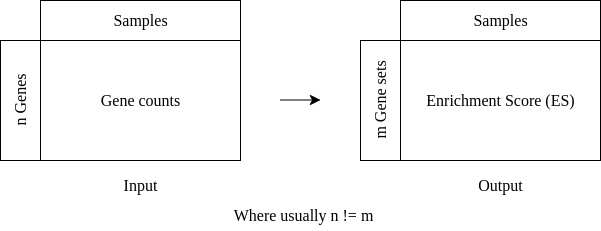
\includegraphics[clip=true,width=7cm]{img/io-gsea.png}
    \caption{GSEA input and output matrices}
    \label{fig:pixels}
\end{figure}

\item Normalize the expression matrix.
\item Sort the gene counts for each sample in descending order.
\item Compute the enrichment score (\ref{eqn:ES}) for every sample and gene set, being the score for each sampled gene ($S_i$)
\begin{equation}
S_i = \sqrt{\dfrac{N - G} {G}}
\label{eqn:EPS}
\end{equation}

if the gene is in the current gene set

\begin{equation}
S_i = -\sqrt{\dfrac{G} {N - G}}
\label{eqn:ENS}
\end{equation}

if it's not.

\begin{equation}
ES = \max_{{1 \leqslant j < N}}\sum_{i=1}^{N} S_i
\label{eqn:ES}
\end{equation}

Where $N$ is the number of sampled genes, $G$ is the size of the current gene set

\end{enumerate}
\vspace{2mm}

\ptitle{Cell clustering}

Clustering is a data analysis method that aims to group similar objects while maximizing the dissimilarity between different groups. In single-cell sequencing experiments, clustering is employed to identify distinct cell populations based on their transcriptional profiles. By partitioning the dataset into subsets of cells that exhibit similar gene expression patterns, clustering allows to uncover hidden structures and relationships within the cellular landscape.

\section{\label{sec:LaTeX} Methods}

\subsection{Rna sequencing}

\ptitle{gseacc}


\ptitle{Limma}



\subsection{}

\begin{figure}[h]
    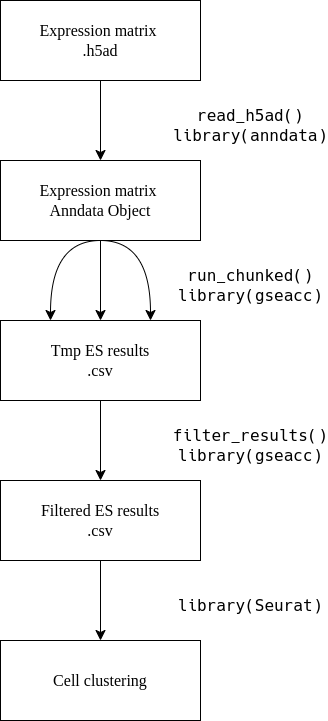
\includegraphics[clip=true,width=4cm]{img/pipeline.png}
    \caption{Scrna-sea pipeline}
     \label{fig:pixels}
\end{figure}

\ptitle{gseacc}

\begin{figure}[h]
    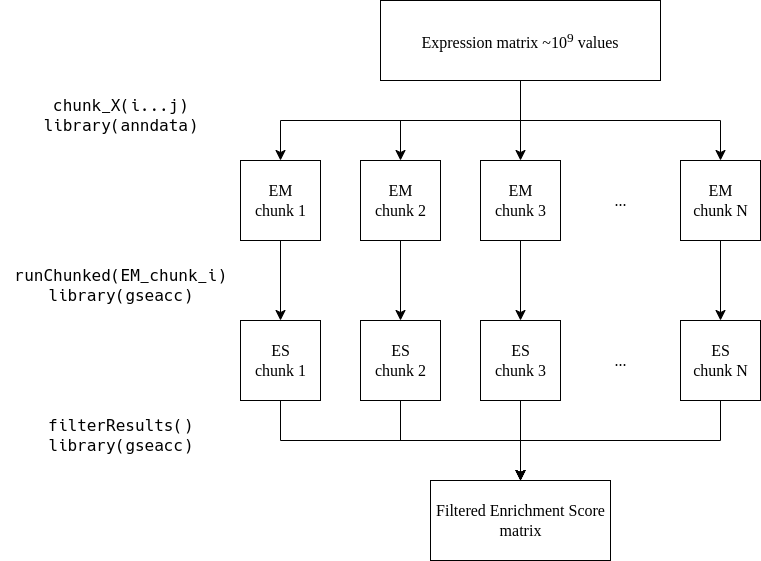
\includegraphics[clip=true,width=7cm]{img/gsea-pipeline.png}
    \caption{Chunked ssGsea for scrna-seq}
     \label{fig:pixels}
\end{figure}


\ptitle{Seurat \cite{seurat-v4} \cite{seurat-web}}

Explain Seurat steps

\section{\label{sec:Results}Results and analysis}

\begin{table}[H]
\centering
\begin{tabular}{ | c | c | }
    \hline
    Processor & Intel® Core™ i5-8250U  \\
    RAM & 8 GB \\
    OS & Ubuntu 23.04 \\
    R version & 4.2 \\
    \hline
\end{tabular}
\caption{Resources used to run all the experiments}
\end{table}


\subsection{RNA-seq}

For the first RNA-seq experiment we used the expression matrix from the GSE121212 experiment \cite{gse121212}. First we obtained the Enrichment Score matrix using gseacc \cite{gse121212-go-es}, and we analysed it using Limma to get the most representing gene sets when comparing different phenotypes.

\begin{table}[H]
\centering
\begin{tabular}{ | c @{\hspace{0.6cm}} c @{\hspace{0.5cm}} c | }
    \hline
    GO term & AveExpr & B \\
    \hline
    \hline
    GO:2000330 & 145.89252 & -3.375500 \\
    GO:0048817 & 94.67299 & -3.396802 \\
    GO:0008973 & 89.61911 & -3.398116 \\
    GO:0032500 & 99.53479 & -3.405704 \\
    GO:0002815 & 99.53479 & -3.405704 \\
    GO:0002805 & 99.53479 & -3.405704 \\
    GO:0032498 & 99.53479 & -3.405704 \\
    GO:0006963 & 99.53479 & -3.405704 \\
    GO:0002807 & 99.53479 & -3.405704 \\
    GO:0002816 & 99.53479 & -3.405704 \\
    \hline
\end{tabular}
\caption{Most different expressed gene sets in Psoriasis non lesional and Psoriasis-lesional}
\end{table}

\subsection{scRNA-seq}



\section{Conclusions}

\bibliography{report}

\end{document}
